% !TeX root = Stageportfolio.tex



\begin{landscape}
	\subsection{Lessen aan VISO}\vspace*{-5mm}
	De bijlagen per lesblok (e.g. bordschema, uitgeschreven oplossingen, labo's \ldots) zijn na elk lesblok terug te vinden. \vspace*{-15mm}
	\subsubsection{Les 11-12}\vspace*{-5mm}
	\begin{tabularx}{1.56\textwidth}{|p{0.35\textwidth}|X|}\hline
		\textbf{Administratieve gegevens}\newline\newline
		Kevin Truyaert\newline\newline
		technisch secundair onderwijs\newline
		3e graad, 1ste jaar, Techniek-Wetenschappen\newline
		VVKSO: \href{http://ond.vvkso-ict.com/leerplannen/doc/Toegepaste\%20fysica-2014-041.pdf}{http://ond.vvkso-ict.com/leerplannen /doc/Toegepaste\%20fysica-2014-041.pdf} \newline
		\underline{Lesonderwerp}:\newline `Labo M4: De stroombalans' & \textbf{Doelstellingen}
		\begin{itemize}[itemsep=0.08\baselineskip]
			\item B24: De richting, de zin en de grootte van de Lorentzkracht op een rechte stroomvoerende geleider aangeven en hiermee de magnetische veldsterkte omschrijven. 
			\item AD4 Reflecteren: Over een waarnemingsopdracht/experiment/onderzoek en het resultaat reflecteren.
			\item AD5 Rapporteren: Over een waarnemingsopdracht/experiment/onderzoek en het resultaat rapporteren.
			\item AD10 Meettoestellen en meetnauwkeurigheid: De gepaste toestellen kiezen voor het meten van de behandelde grootheden en de meetresultaten correct aflezen en noteren.
			\item AD 12 Grafieken: Meetresultaten grafisch voorstellen in een diagram en deze interpreteren.
		\end{itemize}
		\underline{Lesdoelen}\newline
		\vspace{-0.75cm}
		\begin{enumerate}[itemsep=0.08\baselineskip]
			\item De leerlingen kunnen de Lorentzkracht toepassen op de specifieke situatie van de stroombalans.
			\item De leerlingen werken samen om een wetenschappelijke opstelling te kunnen bouwen.
			\item De leerlingen voeren de beschreven handelingen uit om tot resultaten te komen.
			\item De leerlingen werken samen om de metingen uit te voeren.
			\item De leerlingen meten de resultaten nauwkeurig op.
			\item De leerlingen reflecteren over de resultaten.
			\item De leerlingen rapporteren over hun resultaten.
			\item De leerlingen houden bij hun berekeningen rekening met de nauwkeurigheid.
			\item De leerlingen stellen de meetresultaten grafisch voor.
		\end{enumerate} \\\hline
	\end{tabularx}


	\begin{tabularx}{1.56\textwidth}{|p{0.55\textwidth}|X|}
		\hline
		\multirow{2}{0.55\textwidth}{\textbf{Beginsituatie}\newline  
		Er zijn acht leerlingen binnen 5TW. Er heerst een algemene klassfeer. De leerlingen hebben al theorie gekregen  rond en oefeningen gemaakt op de magnetische krachtwerking. \newline\newline Bij dit labo beschikt de school over drie opstellingen van de stroombalans. Er zijn echter maar twee balansen in de school met een nauwkeurigheid van 0.01~g. Ik heb zelf voor een extra balans met nauwkeurigheid van 0.01~g gezorgd, waardoor er drie volledige opstellingen zijn en iedere groep tegelijkertijd aan de slag kan. De mentor voorziet de verdeling van de groepjes, aangezien dit in een rotatiesysteem verwerkt zit voor andere labo's. Er zullen drie groepjes leerlingen zijn.\newline\newline Het lokaal is het fysicalokaal waar mogelijkheid is om elektriciteit uit de  pilaren  die centraal per rij tussen de banken staan. Er zijn voldoende voorzieningen voor het experimentele materiaal. Er is ook een krijtbord en een beamer aanwezig. \newline\newline Dit is mijn eerste les in het tso en is meteen een labo. Als leerkracht ben ik hierdoor wat nerveus (eerste les, labo) maar zeer benieuwd naar het kunnen van de leerlingen, iets wat ik meteen kan testen vanaf mijn eerste les, vanwege het onderwerp. } & \textbf{Acties}\newline  
		- \YellowHighlight{Ik herhaal de theorie die tijdens het labo gebruikt wordt wat door middel van een}{15cm}  \YellowHighlight{korte powerpoint.}{3.3cm} Door deze herhaling zorg ik ervoor dat de beginsituatie voor iedereen terug gelijk is. Dit zal nodig zijn, gezien ik tijdens mijn stage over laatste deel van magnetisme les zal geven, terwijl de vakmentor al bezig is met mechanica. Op die manier zal ik zorgen dat iedereen een voldoende startpunt heeft.\newline\newline
		- \PinkHighlight{Tijdens het labo wil ik bij alle groepjes zeer kort op de bal kunnen spelen.}{13.5cm} Ik acht dit zeer goed mogelijk aangezien er slechts drie groepen zullen zijn. Op die manier kan ik snel bijsturen indien dit nodig kan zijn. Anderzijds kan ik ook hun inzicht testen door hen verdiepingsvragen te stellen rond het onderwerp van het labo. \newline\newline
		- \GreenHighlight{Bij een labo is het de bedoeling om in groep een resultaat op de gestelde onderzoeks-}{15cm} \GreenHighlight{vragen te bekomen.}{3.6cm} Hier worden de leerlingen in drie groepen onder verdeeld. Hierdoor zal er een goede wisselwerking kunnen zijn tussen de leerlingen onderling en zijn er voldoende kritische blikken per groep om de vragen op te lossen. Anderzijds zijn er ook drie opstellingen ter beschikking die voor dit labo gebruikt kunnen worden, waardoor er geen doorschuifsysteem hoeft te ontstaan aangezien het aantal groepen gelijk is aan het aantal opstellingen die ter beschikking zijn. 
		\newline\newline\newline\newline\newline
		
		\\ \cline{2-2}
		  & \textbf{Bronnen}\begin{itemize}
		  	\item Schramme, S. (2018) De stroombalans, labo magnetisme 4
		  	\item Frederiksen (2014), Current Balance 4565.00
		  \end{itemize}\\ \hline
	\end{tabularx}


\newpage
	
	\begin{tabularx}{1.56\textwidth}{|p{1.5cm}|p{7cm}|X|p{4cm}|}
		\hline
		\textbf{Nr. lesdoel } & \textbf{Inhoud (timing)}  & \textbf{Organisatie } & \textbf{Media } \\ \hline
		&\underline{Korte voorstelling (5 minuten)}\newline
		Tijdens deze lesfase wil ik mezelf kort voorstellen, aangezien dit mijn eerste les aan deze klas is. Ik vraag hen om een naamkaartje te plaatsen. Gezien er slechts acht leerlingen zijn, hoop ik dat ik die niet lang nodig heb.
		&  \underline{Vertellen}\newline 
		Ik vermeld mijn naam en schrijf die op het bord.
		& Krijtbord 
		\\ \hline
	\end{tabularx}

\begin{tabularx}{1.56\textwidth}{|p{1.5cm}|p{7cm}|X|p{4cm}|}
	\hline
	\textbf{Nr. lesdoel } & \textbf{Inhoud (timing)}  & \textbf{Organisatie } & \textbf{Media } \\ \hline
	1&\underline{Korte herhaling theorie Lorentz-} \underline{kracht + inleiding labomagnetisme 4:} \underline{de stroombalans (15 minuten)}\newline
	Ik begin met de opstelling van dit labo te bespreken. Dit doe ik aan de hand van het stappenplan dat de leerlingen ook zullen moeten volgen om de opstelling te bouwen. Op dit moment weten ze dus nog niet wat ze hiermee zouden willen meten, wat ik hen hierna expliciet vraag. \newline
	Aangezien dit labo over de Lorentzkracht zal gaan, herhaal ik die kort en bespreek ik de factoren van de formule nog eens duidelijk. Daarna stap ik terug met de Lorentzkracht naar de onderzoekssituatie, om zo tot de onderzoeksvragen te komen. 
	&  \underline{Onderwijsleergesprek + vertellen}\newline 
	Ik vertel het stappenplan samen met de leerlingen op, om hen daarna te laten nadenken over het mogelijke doel van dit labo. Hier kunnen interessante antwoorden op komen, waar we samen op zoel kunnen gaan of dit ook zo mogelijk zou zijn. Wanneer ik `Lorentzkracht' hoor vallen, zal ik samen met de leerlingen dit nog eens kort herhalen om daarna met hen dit naar het onderzoek terug te koppelen. 
	Ik overloop de onderzoeksvragen en vertel hen hoe ze hun metingen zullen verrichten.
	
	
	& Slides (zie bijlage deze les) 
	\\ \hline
\end{tabularx}



\begin{tabularx}{1.56\textwidth}{|p{1.5cm}|p{7cm}|X|p{5cm}|}
	\hline
	\textbf{Nr. lesdoel } & \textbf{Inhoud (timing)}  & \textbf{Organisatie } & \textbf{Media } \\ \hline
	2&\underline{Bouwen opstelling (10 minuten)}\newline
 		Tijdens deze lesfase is het belangrijk dat de leerlingen samen werken en elkaar aanvullen om de opstelling te bouwen en te begrijpen. 
	&  \underline{Onderzoekspracticum}\newline 
	De leerlingen bouwen zelfstandig hun opstelling op aan de hand van de beschreven stappen in hun labobundel (Zie pagina 3 van de bundel). Ondertussen loop ik rond om hen te controleren en vragen te stellen rond het onderwerp. Wanneer de leerlingen klaar zijn, vragen ze mij om de opstelling te controleren vooraleer ze de metingen mogen starten.
	& Onderzoeksbundel \newline\newline Tweemaal opstelling:
	\begin{itemize}
		\item Stroombalans
		\item Stroombron
		\item Balans 0.01g
		\item Ampèremeter
		\item Statief en statiefklem
		\item Verbindingskabels
	\end{itemize}
	\\ \hline
\end{tabularx}



\begin{tabularx}{1.56\textwidth}{|p{1.5cm}|p{7cm}|X|p{5cm}|}
	\hline
	\textbf{Nr. lesdoel } & \textbf{Inhoud (timing)}  & \textbf{Organisatie } & \textbf{Media } \\ \hline
	1\newline\newline 3\newline\newline 4\newline\newline 5\newline\newline 6&\underline{Onderzoeksvragen (35 minuten)}\newline
		De leerlingen voeren de metingen horende bij de onderzoeksvragen uit.
	&  \underline{Onderzoekspracticum}\newline 
	Eens de opstellingen goedgekeurd zijn, kunnen de leerlingen beginnen aan het uitvoeren van de metingen om de onderzoeksvragen te beantwoorden. Hiervoor zullen de leerlingen minstens dertien verschillende metingen moeten uitvoeren.
	& Onderzoeksbundel \newline\newline Driemaal opstelling
	\\ \hline
\end{tabularx}

\begin{tabularx}{1.56\textwidth}{|p{1.5cm}|p{7cm}|X|p{5cm}|}
	\hline
	\textbf{Nr. lesdoel } & \textbf{Inhoud (timing)}  & \textbf{Organisatie } & \textbf{Media } \\ \hline
	 6\newline\newline 7\newline\newline 8\newline\newline 9&\underline{Rapporteren en grafieken in Excel} \underline{maken (33 minuten)}\newline
	De leerlingen beginnen aan het schrijven van hun rapport in de bundel. Ze maken grafieken in excel om hun vergelijkingen te bekomen. Ze houden rekening met de nauwkeurigheid van hun metingen bij het maken van verdere berekeningen.
	&  \underline{Onderzoekspracticum}\newline 
	De leerlingen gaan naar het coomputerlokaal om hun gemeten data te verwerken tot grafieken. Deze grafieken drukken ze af en voegen ze toe aan hun bundel. Daarnaast evalueren ze zichzelf op enkele criteria (eerste blad bundel), die uitgebreider vermeld zijn op bladen die ze in het begin van het jaar gekregen hebben. Deze komen overeen met de algemene doelstellingen die in het leerplan vermeld zijn.\newline\newline De leerlingen zullen hiermee nog niet klaar zijn op het einde van de les en doen hiermee volgende les (4 maart) verder. Ik verwacht dat ze grafieken van hun opgemeten data klaarhebben en daarmee op de voorlaatste pagina van hun bundel zitten.
	& Onderzoeksbundel \newline\newline Driemaal opstelling\newline\newline Computerlokaal
	\\ \hline
\end{tabularx}
%	
\newline
\newline

\begin{tabularx}{1.56\textwidth}{|p{1.5cm}|p{7cm}|X|p{5cm}|}
	\hline
	\textbf{Nr. lesdoel } & \textbf{Inhoud (timing)}  & \textbf{Organisatie } & \textbf{Media } \\ \hline
	1\newline\newline 6&\underline{Afsluiten (2 minuten)}\newline 
	&  \underline{Afsluiten}\newline
	Ik herhaal samen met de leerlingen nog eens mondeling wat hun bevindingen van dit labo waren.
	& 
	\\ \hline
\end{tabularx}
	
%	
	
	
\end{landscape}


%\subsection*{Bijlage 5.1: slides introductie}

\includepdf[scale = 0.9, pages = -,pagecommand=\subsection*{Bijlage 5.1: slides introductie},nup=2x3, delta = 0.5cm 1cm]{LaboM4.pdf}
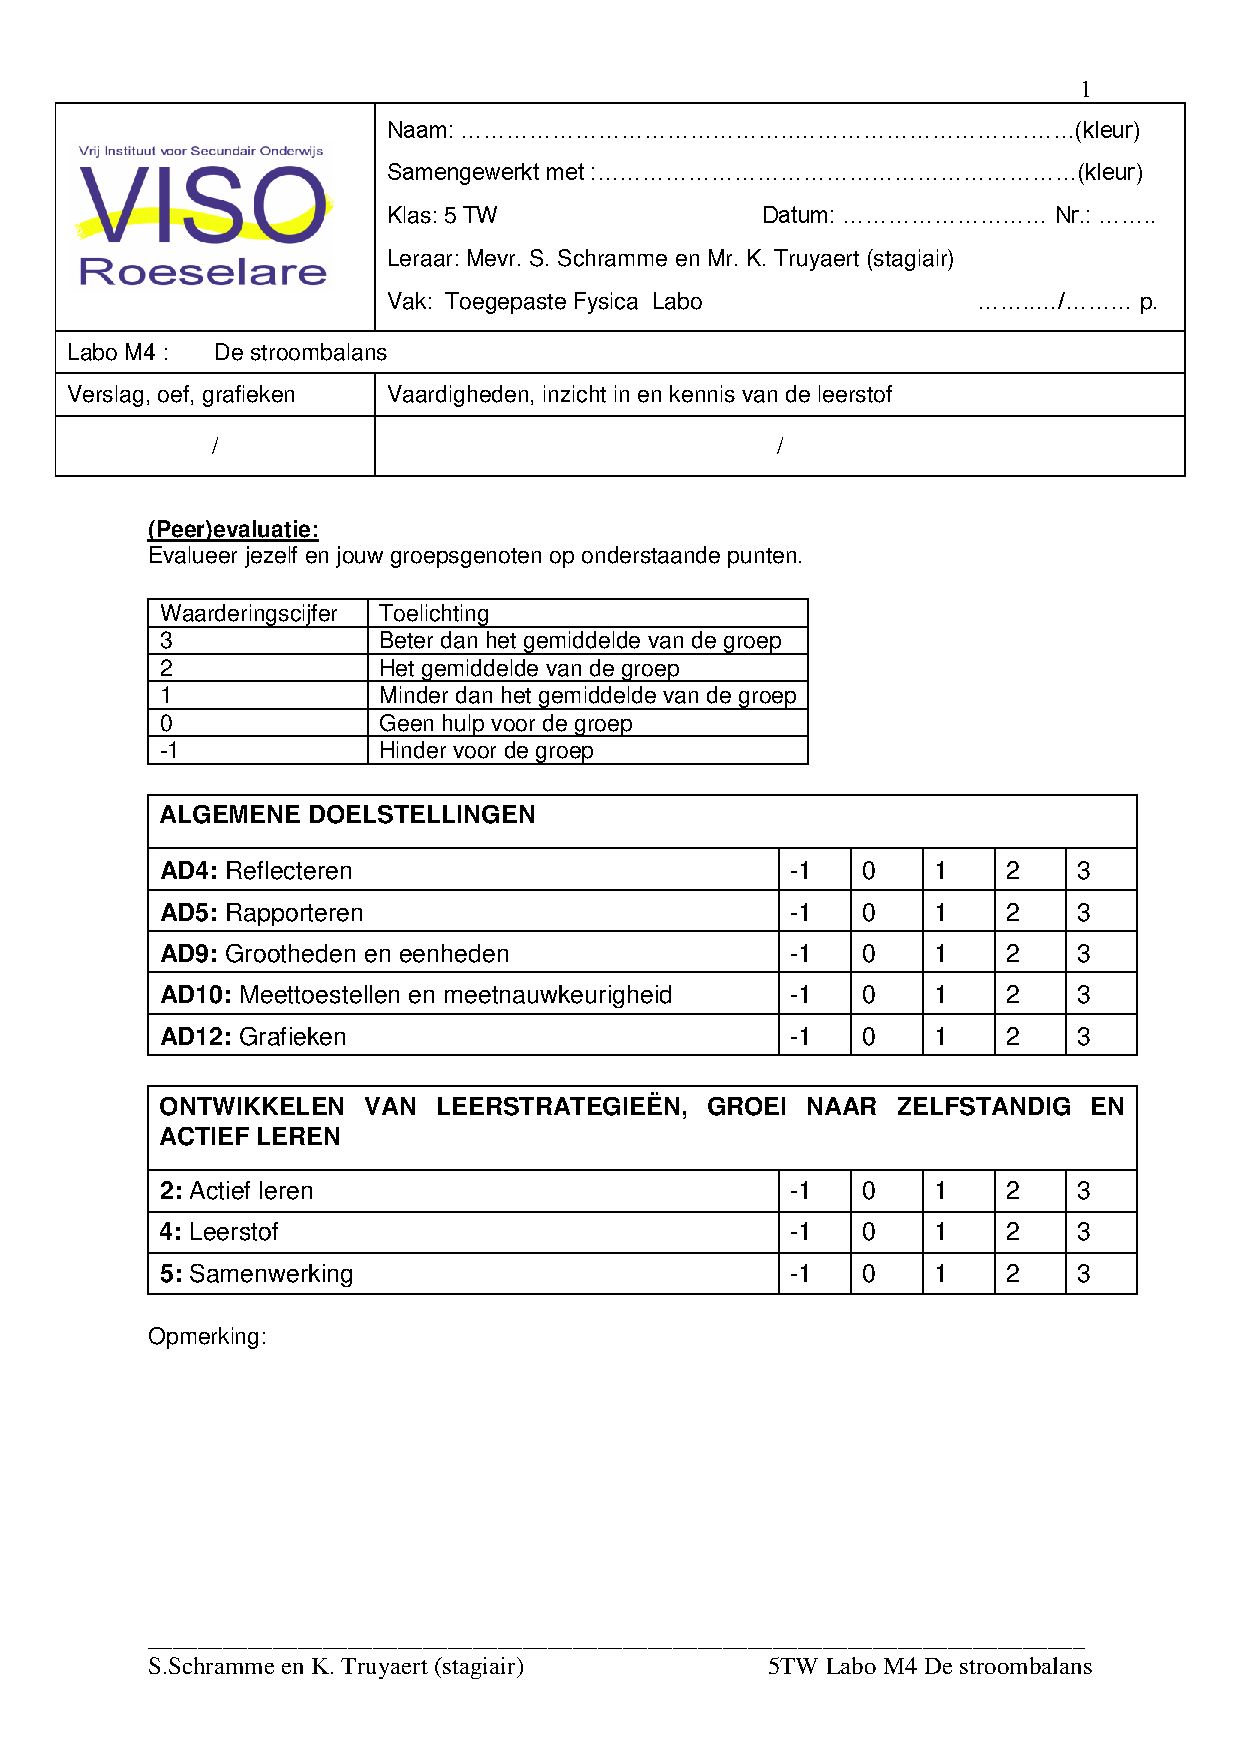
\includepdf[scale = 0.9, pages = 1,pagecommand=\subsection*{Bijlage 5.2: onderzoeksbundel over `De stroombalans'}]{M4Stroombalans1920.pdf}
\includepdf[scale = 0.9, pages = 2-,pagecommand=]{M4Stroombalans1920.pdf}

%
%\subsection*{Bijlage 1.2: bordschema theorie}
%\begin{center}
%	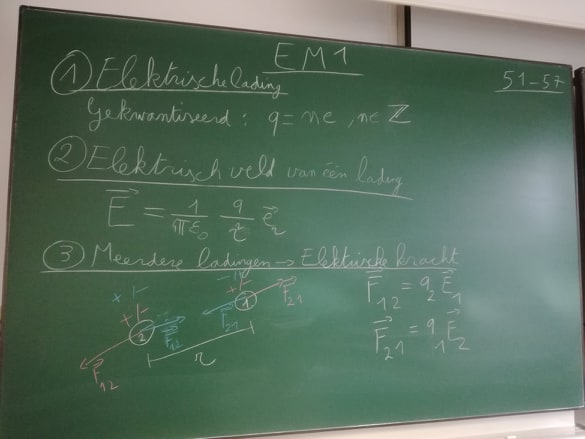
\includegraphics[width=0.9\textwidth]{Bord1a}
%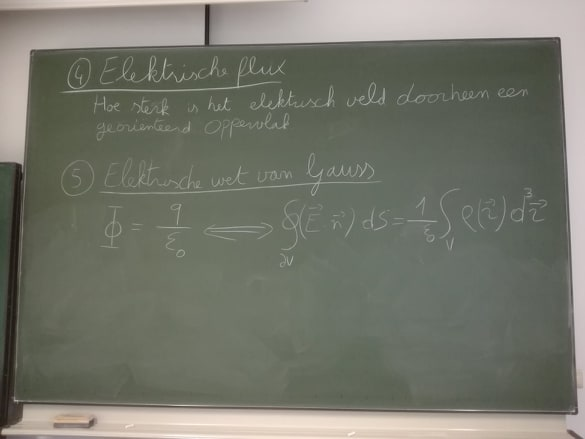
\includegraphics[width=0.9\textwidth]{Bord1b}
%\end{center}
%\newpage
%
%
%\includepdf[scale = 0.8,pages = 17,pagecommand=\subsection*{Bijlage 1.3: opgeloste oefeningen}]{Observaties_OpgelosteOef}
%\includepdf[scale = 0.8,pages =18-20,pagecommand=]{Observaties_OpgelosteOef}
%
%
%
%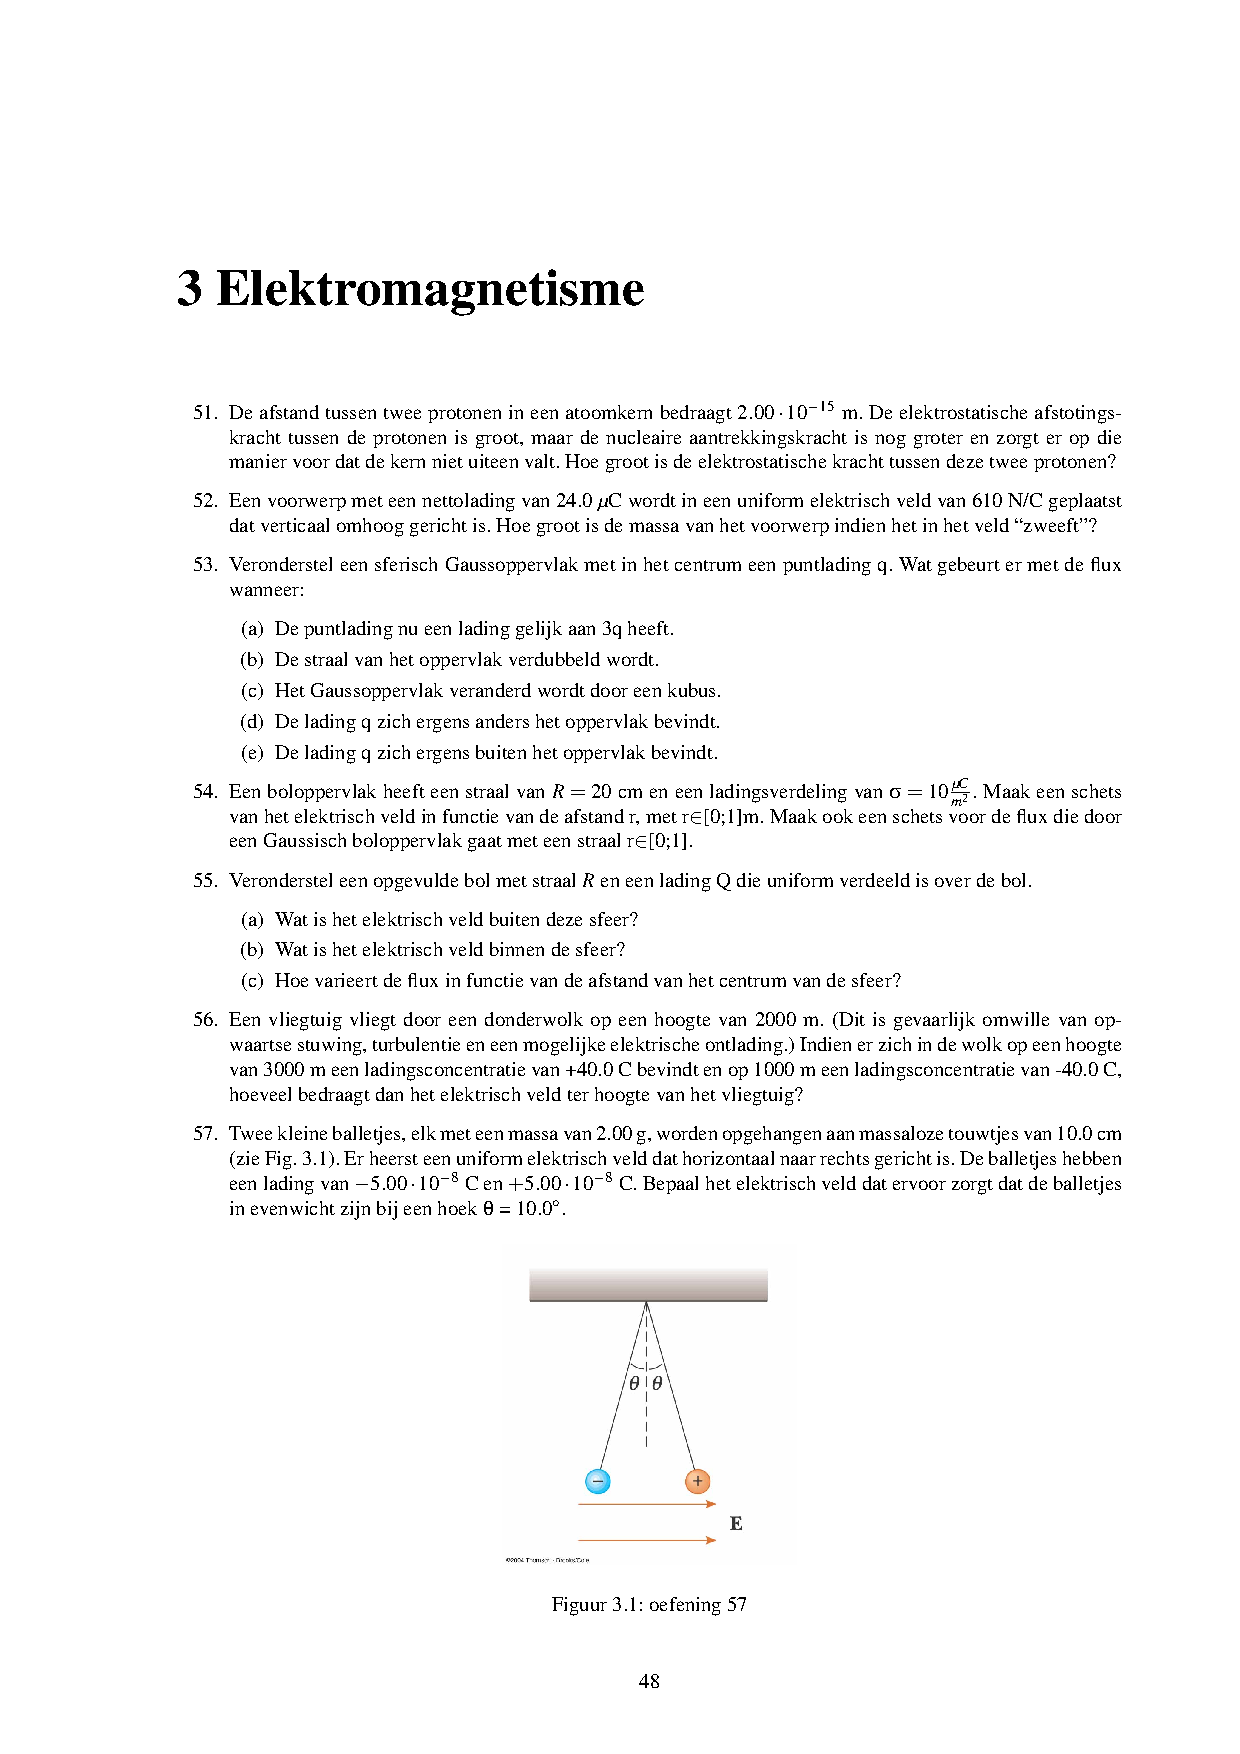
\includepdf[scale = 0.95,pages = 1,pagecommand=\subsection*{Bijlage 1.4: oefeningenbundel elektromagnetisme}]{OefeningenBundel}
%\includepdf[scale = 0.95,pages =2-,pagecommand=]{OefeningenBundel}